\documentclass[11pt, aspectratio=169]{beamer}

% LuaLaTeXで日本語を使うための必須パッケージ
\usepackage{luatexja}

% 便利な追加パッケージ
\usepackage{booktabs}   % 表の罫線
\usepackage{tikz}       % 図形描画
\usepackage{graphicx}
\usepackage{listings}   % ソースコード挿入
\lstset{
  basicstyle=\ttfamily\scriptsize,
  frame=single,
  breaklines=true,
  numbers=left,
  numberstyle=\tiny
}

% テーマとカラーテーマの設定
\usetheme{Madrid}
\usecolortheme{orchid}

% ==========================================
% 【改良】セクション・サブセクションの可視化設定
% ==========================================

% 1. セクション開始時の自動表紙（大きな扉絵）
\AtBeginSection[]{
  \begin{frame}
    \vfill
    \centering
    \begin{beamercolorbox}[sep=8pt,center,shadow=true,rounded=true]{title}
      \usebeamerfont{title}\insertsectionhead\par%
    \end{beamercolorbox}
    \vfill
  \end{frame}
}

% 2. サブセクション開始時に「現在のセクション内の目次」を自動挿入
% 今いるサブセクション以外を半透明（shaded）にすることで、現在地が強調されます
\AtBeginSubsection[]{
  \begin{frame}{\insertsectionhead}
    \tableofcontents[currentsection, currentsubsection, subsectionstyle=show/shaded/hide]
  \end{frame}
}

% タイトル情報
\title{妨害通信の数理とシミュレーション環境の構築}
\subtitle{妨害通信}
\author{学籍番号(Student ID): 1280391 \\ 氏名(Name): 細川夏風(Hosokawa Natsuka)}
\institute{高知工科大学(Kochi Univ of Tech)}
\date{\today}

\begin{document}

% タイトルスライド
\begin{frame}
  \titlepage
\end{frame}

% 全体目次スライド
\begin{frame}{目次}
  \tableofcontents
\end{frame}

% ==========================================
% ここから本文
% ==========================================

\begin{frame}{進捗}
  \begin{enumerate}
    \item \texttt{SAGIN}の通信妨害
    \item \texttt{SAGIN}の概要
    \item 通信妨害と概要
    \item 通信妨害の数理(今回)
  \end{enumerate}
\end{frame}

\section{妨害通信の数理}
\subsection{前提知識}

\begin{frame}{妨害通信を学ぶに当たって}
  % ここに内容を記述
  \begin{itemize}
    \item \textbf{最尤函数} $f(y|s)$ \\
      受信信号$y$が与えられたとき，送信信号$s$がどのような値がもっともらしいかを表した函数
    \item \textbf{特性函数} \\
      線形和の変数を$1$つの指数の線形和の形に変形する
    \item \textbf{\texttt{Q}函数} $Q(x)$\\
      入力値$x$から$\infty$までの標準正規分布の積分
    \item \textbf{\texttt{BPSK}} \\
      現在用いられている通信方式，$1$が来たらある電圧$A$と認識，$0$が来たらある電圧$-A$と認識する
  \end{itemize}
\end{frame}

\subsection{信号の認識}

\begin{frame}{通信からもっともらしさを}
  すべての送信シンボル$\forall s \in S$の事前確率が等しい場合，受信信号$y$が与えられたとき，最尤函数を用いて得られた$y$がを推定．
  \begin{align*}
    \hat{s} = \arg \min \limits_{s \in S} |y - s| ^2
  \end{align*}
  最終的に$2$点間の距離の最小化に帰着する．難しく書いているが，得られた値が$1$と$0$のどちらに近いかという単純な式．
\end{frame}

\subsection{ノイズの集約}

\begin{frame}{ノイズ同士の関係}
  通常の通信の際に発生するノイズ(\texttt{AWGA})と妨害者が発生させるノイズが存在する．これらと送信信号は受信側では線形の関係にあり，受信信号$y$，送信信号$s$，自然に発生するノイズ$w$，妨害者のノイズ$z$は以下の式で表せる．このとき，ノイズはガウス分布に従うものとする．
  \begin{align*}
    y = s + w + z
  \end{align*}
  この式に対して，特性函数$\varphi$を用いると$2$つのノイズ$\mathcal{N}(0, \sigma^2) = \mathcal{N}(0, \sigma_w^2 + \sigma_z^2)$と表すことができる．
\end{frame}

\subsection{妨害}

\begin{frame}{妨害による情報の喪失(1)}
  前述の$Q$函数を用いて，妨害電波が極限$\lim \limits_{\sigma_z^2 \rightarrow \infty}$まで近づいた場合を考える．
  \begin{align*}
    \lim \limits_{\sigma_x^2 \rightarrow \infty} P_e &= \lim \limits_{\sigma_x^2 \rightarrow \infty} Q \left( \frac{A}{\sqrt{\sigma_w^2 + \sigma_z^2}} \right) \\
    &= Q(0) \text{に収束し} \\
    & \int_{- \infty}^{\infty} \frac{1}{\sqrt{2 \pi}} \exp \left( - \frac{u^2}{2}\right) du = 1 \text{より，その半分}\frac{1}{2}\text{となる}
  \end{align*}
\end{frame}

\begin{frame}{妨害による情報の喪失(2)}
  シャノン=ハートレーの定理から
  \begin{align*}
    C &= \lim \limits_{\sigma_z^2 \rightarrow \infty} \log \left(1 + \frac{A^2}{\sigma_w^2 + \sigma_z^2} \right) \\
    &= \log_2(1) \\
    &= 0
  \end{align*}
  となり，情報が失われることがわかる．
\end{frame}

\begin{frame}{図で見る}
  \begin{figure}[htpb]
    \center
    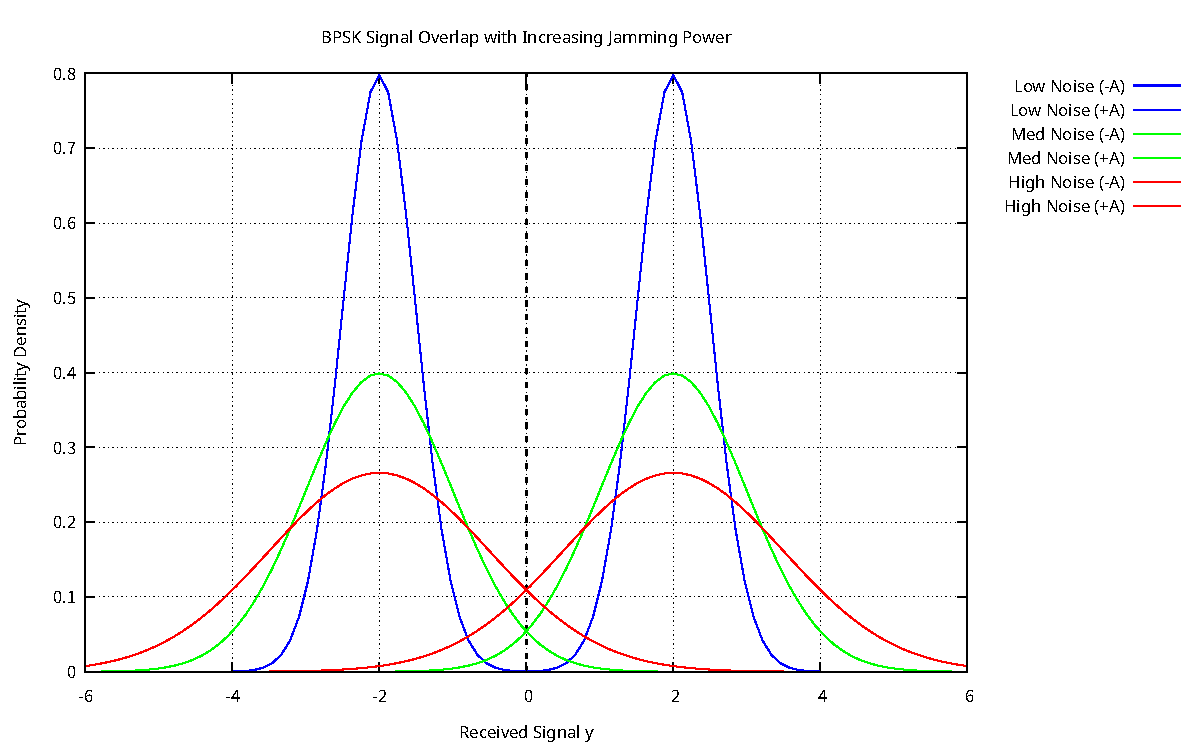
\includegraphics[width=10.5cm]{jamming_merged.pdf}
    \caption{それぞれの妨害の影響}
  \end{figure}
\end{frame}

\subsection{まとめ}

\begin{frame}{まとめ}
  \begin{block}{妨害はノイズの強度}
    以上の簡易的な証明と図示により，妨害はノイズの強度に大きく依存していることがわかる．妨害電波が強ければ強いほど通信に支障をきたし，弱いと明瞭に通信を行うことが可能である．
  \end{block}
\end{frame}

\section{サーバへの環境構築}

\begin{frame}{環境構築}
  以前から計画した\texttt{Pyjama}を\texttt{shikharlab-01}のサーバへ環境構築を行った．ホームディレクトリの直下に\texttt{jamming\_env}というディレクトリを生成し，その中に\texttt{Dockerfile}，\texttt{docker-compose.yml}のファイルをおいている．各々，サーバへの接続は\texttt{ssh}で行ってもらい，その後のコンテナ内への接続等はターミナル，もしくは\texttt{VScode}で行うことを想定している．\texttt{Jupyter}形式のため，\texttt{VScode}を推奨する．また，\texttt{Jupyter}への接続としてサーバにおけるローカルに$8080$ポートを解放している．ただし，リモート環境のため動作が異なる可能性が高い．
\end{frame}

\section{今後の学習予定}

\begin{frame}{今後の学習予定}
  \begin{itemize}
    \item 魏先生の輪講で強化学習を勉強
    \item 強化学習で用いるかつ妨害手法と対策手法の活用予想に用いるためゲーム理論を勉強

    \vspace{1em}

    \item 簡易的な妨害を行う\texttt{Python}プログラムの作成
  \end{itemize}
\end{frame}

\section{参考文献}

\begin{frame}[allowframebreaks]{参考文献}
  \begin{thebibliography}{9}
    \setbeamertemplate{bibliography item}[book]
    \bibitem{shannon}
      C. E. Shannon, "A Mathematical Theory of Communication," 
      \textit{Bell System Technical Journal}, 1948.
      
    \setbeamertemplate{bibliography item}[article]
    \bibitem{survey}
      H. Zeng et al., "Jamming Attacks and Anti-Jamming Strategies in Wireless Networks: A Comprehensive Survey," 
      \textit{IEEE Communications Surveys \& Tutorials}, 2024.
      
    \bibitem{sagin}
      K. Yang et al., "Communications in Space–Air–Ground Integrated Networks: An Overview," 
      \textit{Space: Science \& Technology}, 2025.
      
    \bibitem{ew_future}
      天貝 崇樹, "次世代の電子戦について ― 機械学習とネットワークを活用した EMS 活動 ―," 
      \textit{防衛技術ジャーナル}, 2020.
      
    \bibitem{security}
      M. Harvanek et al., "Survey on 5G Physical Layer Security Threats and Countermeasures," 
      \textit{Sensors}, 2024.
  \end{thebibliography}
\end{frame}

\end{document}
